\documentclass{article}
\usepackage{fixltx2e}
\usepackage{graphicx}
\title{Improper Integrals}
\author{Sriram Vadlamani}
\begin{document}
\maketitle
\newpage
\tableofcontents
\newpage
\section{Definition}
We call a sequence of functions from I $\rightarrow$ R defined by $(f_{n})_{n \in N}$ $\in$ $(R^{I})^{N}$\\
Below we can see an example of what a sequence of functions looks like.\\
The function defined is $f_{n} (x)$ = $ \frac{sin(n \cdot x)}{x} $ \\
We can see the sine wave vary from each n value.\\
\begin{center}
	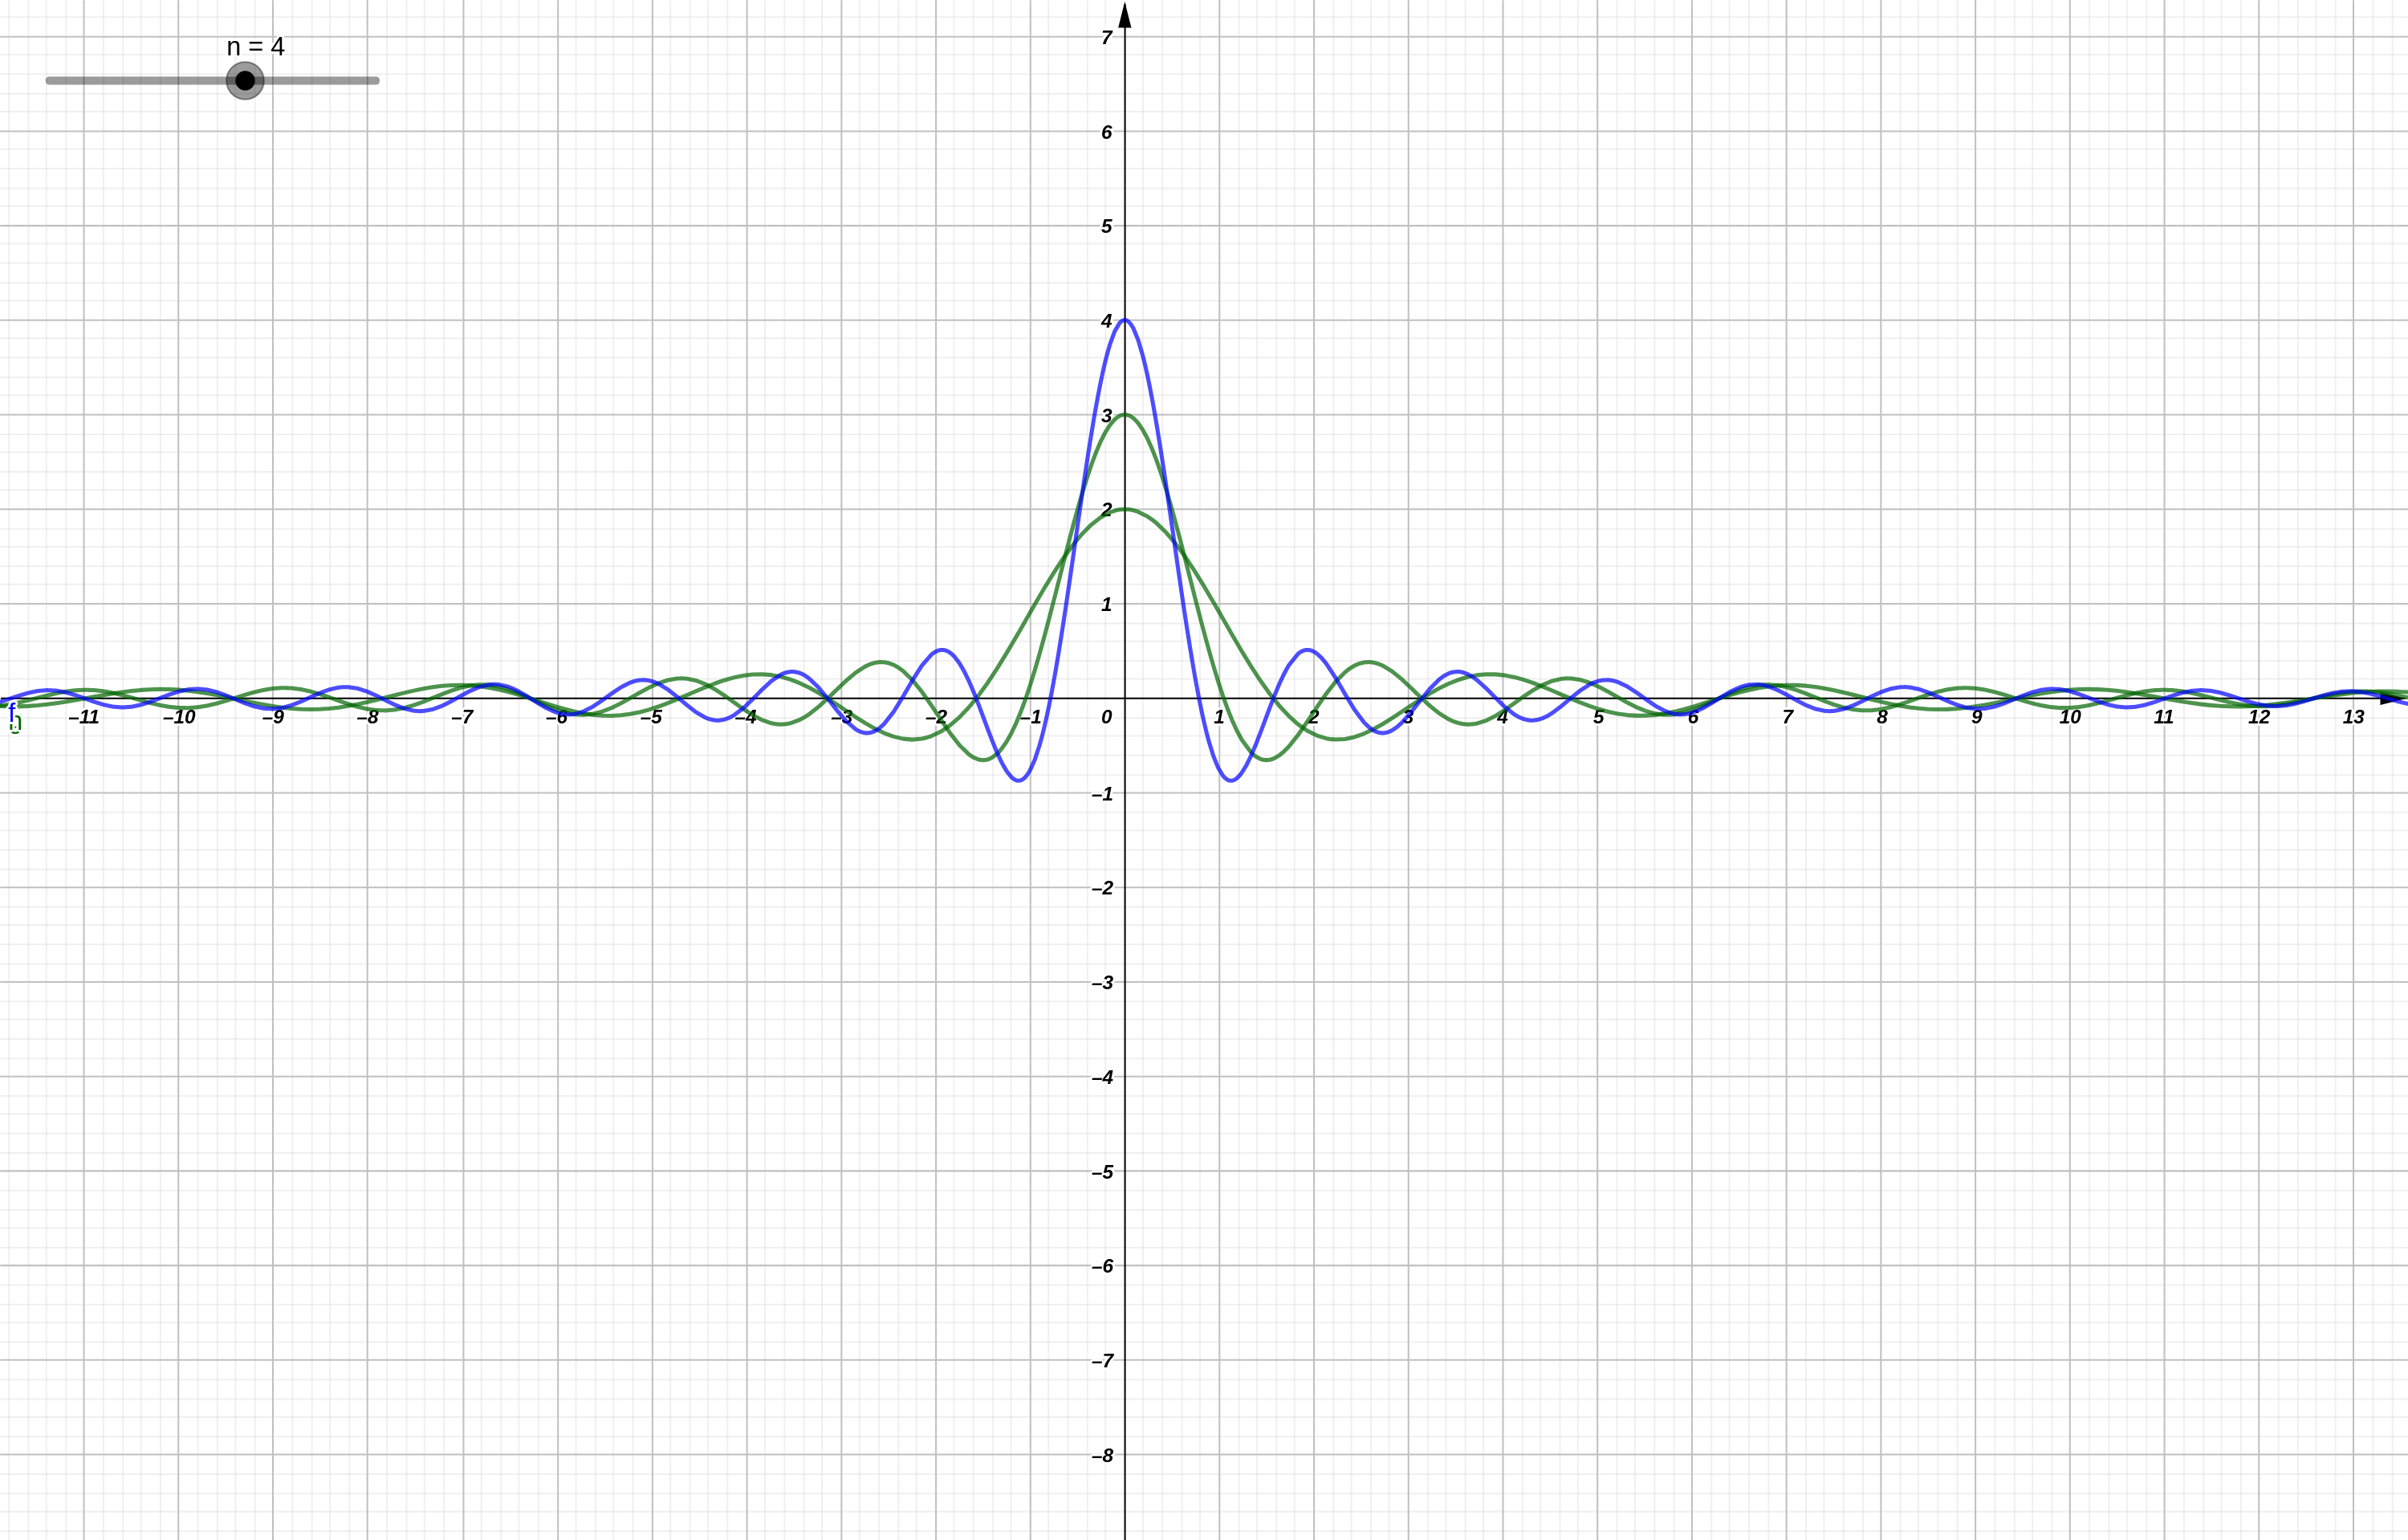
\includegraphics[scale=0.55]{functionSequence.png}
\end{center}
\section{Convergence}
\subsection{Point Wise Convergence}
We say that a sequence $(f_{n})$ is pointwise convergent if:\\
$\displaystyle\lim_{n \to +\infty} f_{n} (x) = f(x)$\\
This goes to say that the sequence has to converge to a function \textit{f} from the same input set \textit{I}.\\
\textbf{Example:}\\
$f_{n}$ : $\left\{ \begin{array}{c}[0,1] \longmapsto \mathbb{R} \\ x \longmapsto x^{n} \end{array}\right.$\\
setting $x = 0$ or $x = \frac{1}{2}$ we get $\displaystyle\lim_{n \to +\infty}$ $f_{n} (x) = 0$\\
But if x is 1, then the limit is 1 and it converges to that function.\\
Basically, for any given value of \textit{x} we check the limit when \textit{n} reaches infinity, and if it's zero, it's pointwise convergent.\\
\subsection{Uniform Convergence}
\textbf{Definition} let $f_{n}$ and $f \in \mathbb{R}^{I} $ be the function sequence and the limit respectively. We say that $f_{n}$ is uniformly convergent, 
if for any given value of n, the supremum $\mid f_{n} (x) - f(x) \mid$ exists and the supremum (which is a numerical sequence) has to tend to zero around positive infinity.\\
\textbf{Example}
\end{document}
